% Chapter Name
\chapter{\sc Polymorphic Graphene: Modulating the Graphene Surface Structure}
\label{ch:Polymorphic Graphene}
\section{Graphene on Ruthenium: a departure from pristine graphene}

Chapter 2 discussed the properties of graphene in its ideal form, a perfect two-dimensional hexagonal crystalline lattice of carbon atoms. However, when graphene is grown on various substrates its material properties and structure can manifest in drastically different ways. Graphene growth on metallic substrates has been widely studied and generally the properties of the system can be separated into two categories: systems with weak carbon-metal interaction, such as graphene on gold, and systems with strong carbon-metal interaction, such as graphene on ruthenium \cite{batzill, graphene-metals}.

\begin{figure}

\centering

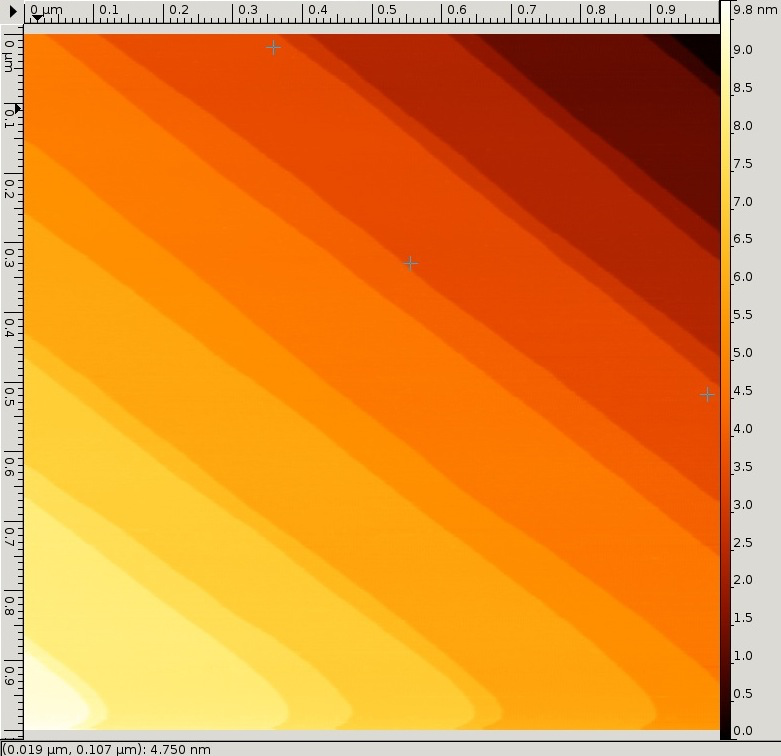
\includegraphics[scale=0.5]{./figs/ru-stm-clean.png}

\caption{
STM image showing the surface of a well prepared ruthenium (0001) single crystal. The surface exhibits atomically flat terraces separated by monatomic steps. Image dimensions are 1$\mu$m x 1$\mu$m.
}
\label{fig:ru-stm-clean}

\end{figure}

Ruthenium is a transition metal with a hexagonal crystal structure and lattice constant of 2.7 {\AA}. The most common applications for ruthenium are principally restricted to electronic use as a hardening agent in electrical contacts as well as a resistive material in its native oxide state, \ce{RuO_2} \cite{ru-electronics, ru-resistors}. However, ruthenium is also used in smaller quantities for catalytic properties as well as in some novel dye-sensitized photovoltaic applications \cite{ru-solar}. The (0001) surface of ruthenium consists of atomically flat terraces with hexagonal surface symmetry terminated by monatomic steps where the atoms in the lower terrace have a $180^{\circ}$ rotation relative to the top terrace. A large scale STM image of a clean ruthenium surface is shown in Figure \ref{fig:ru-stm-clean}.

The most common lattice defects in ruthenium crystals constitute oxygen, sulfur, and carbon. All non-carbon defects can be easily removed from the crystal via prolonged high temperature annealing \cite{ru-auger-prep}. Carbon, however, is not removed in this cleaning process and thus additional methods are required to prepare a pristine ruthenium single crystal. Two methods are commonly employed to prepare pristine ruthenium. First, the crystal may be cleaned by repeated cycles of ion sputtering and annealing. Generally argon ions are used as the sputtering agent. This method leaves the surface area free of contaminants but also has a tendency to leave subsurface pockets of argon atoms, which are visible in STM images. If sputtering is not used, then carbon can be removed from the ruthenium bulk by repeated cycles of exposure to oxygen followed by high temperature annealing. This process works as a result of the variability of carbon solubility in the ruthenium crystal as a function of temperature.

At elevated temperatures, the bulk carbon solubility drops, resulting in a diffusive flow of interstitial carbon atoms from the bulk region to the surface. When the surface is exposed to oxygen, carbon atoms bond with oxygen atoms to produce \ce{CO} molecules. Upon annealing, the carbon monoxide molecules desorb from the surface to vacuum. Thus repeated cycles of oxygen exposure and annealing will deplete the bulk crystal of carbon contaminants. This process can be monitored with Auger electron spectroscopy in order to determine the relative carbon concentration in the crystal. The Auger signal for carbon in ruthenium crystals is somewhat complicated compared to the other contaminants due to the strong overlap between the ruthenium signal and carbon signal near 273 eV. By examining the differentiated auger spectrum, a clean ruthenium sample is characterized by a roughly symmetric peak and trough near 273 eV whereas a largely carbon contaminated sample will manifest with a largely reduced peak and extended trough at 273 eV \cite{ru-auger-prep}. 

\begin{figure}
\centering
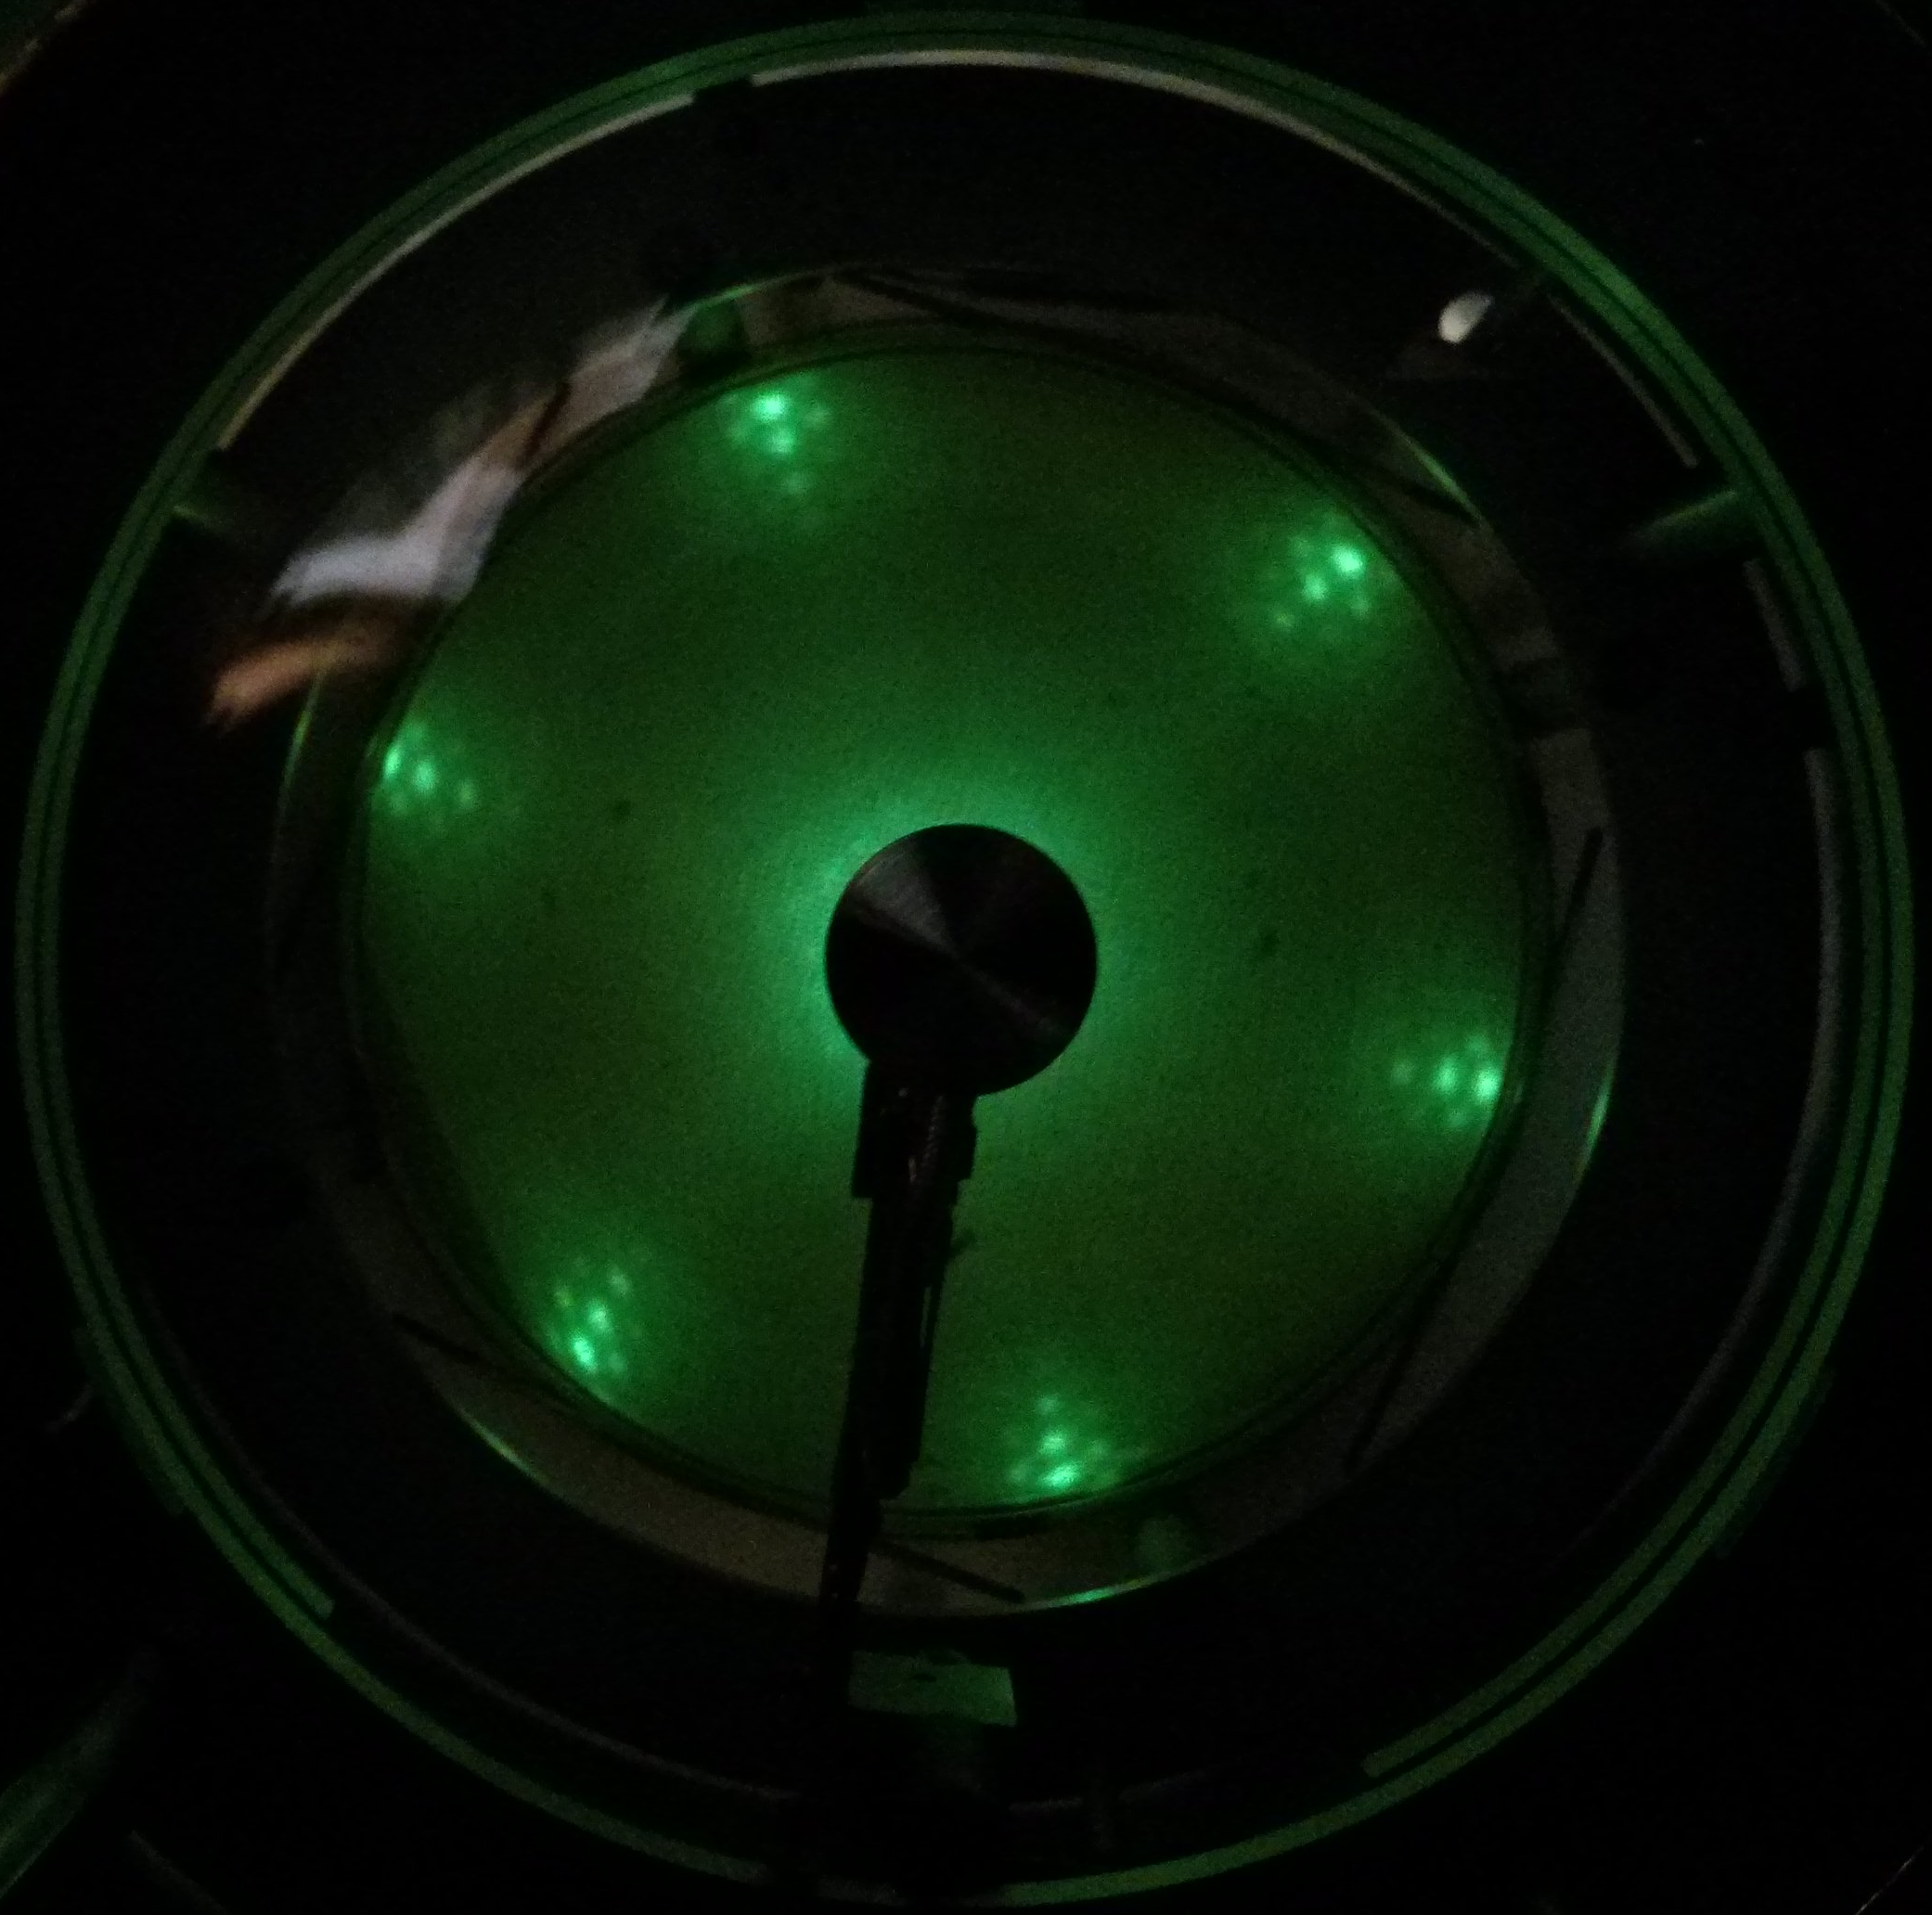
\includegraphics[scale=0.20]{./figs/graphene-ruthenium-leed.png}
\caption{
LEED pattern of the graphene/ruthenium system displaying characteristic satellite peaks surrounding the primary ruthenium (1x1) pattern. Image collected with incident beam energy of 62 eV. The bright diffraction peaks in the center of the outer hexagons represent the ruthenium p(1x1) pattern. The surrounding diffraction spots, referred to as satellite peaks, indicate the presence of the moire superstructure. 
}
\label{fig:graphene-leed}

\end{figure}


A clean ruthenium (0001) crystal can be characterized by an auger signal displaying only strong ruthenium peaks with little contribution from oxygen, carbon, and sulfur. A sample Auger spectrum with from clean ruthenium can be seen in Figure \ref{fig:auger-ru}; the primary peak is roughly symmetric at 273 eV indicating low carbon contamination and the oxygen peak at 512 eV is negligible.  Furthermore, for a clean ruthenium crystal, the LEED pattern will display only a (1x1) primary hexagonal structure, which will be visible in conventional LEED between 50 - 60 eV. If residual oxygen is present in the system from the cleaning cycles, it will be easily visible as a p(2x2) LEED structure. Residual surface carbon from cleaning cycles or from prolonged high temperature annealing can also be clearly distinguished by its LEED signature.

Surface carbon on ruthenium (0001) readily forms graphene islands via a two-step process. When a diffusive flow of carbon is driven from the bulk to the surface by thermal annealing, the carbon atoms first manifest as surface adatoms in a disordered phase. Continued annealing drives the transition from amorphous carbon adatoms to an ordered graphene phase. In this process carbon atoms join into rings forming a graphene structure. However, it should be noted that the growth process of graphene on ruthenium is not as simple as the process on other materials. At the ruthenium surface there is a large energy barrier inhibiting the transition of carbon adatoms into ordered graphene \cite{c-clusters}. LEEM and DFT studies attribute this barrier to the change in height when transitioning from a carbon adatom to a carbon atom in a graphene sheet above the surface \cite{c-clusters}. Instead of a direct transition, it is energetically favorable to form clusters of five carbon atoms that then combine with the graphene sheet edge. This type of growth process is characteristic of metal-carbon systems exhibiting strong metal-carbon bonds, such as graphene on nickel \cite{c-clusters}.

The combination of a hexagonal graphene surface layer atop the hexagonal ruthenium crystal results in an interesting phenomenon known as a moire structure. Both crystal systems are hexagonal and have similar but not perfectly matched lattice constants, with a percent difference of roughly 9\%. As a result of the lattice mismatch, the graphene layer does not lie flat atop the ruthenium surface. Instead, a rippled periodic superstructure forms. The rippled carbon surface also causes pronounced changes in the atomic positions of the uppermost ruthenium surface layers; the uppermost ruthenium layers also exhibit rippled deviations from their normal bulk positions \cite{sxrd}.  The size of the superstructure can be revealed by its reciprocal space pattern imaged with LEED \cite{graphene-metals}. 

The moire structure in LEED for the graphene/ruthenium system is characterized by sharp satellite peaks that form a hexagon surrounding the primary substrate peaks as shown in Figure \ref{fig:graphene-leed}. The ratio between the primary substrate hexagonal reciprocal lattice constant and the satellite peak reciprocal lattice constant is reported to be 11.6 \cite{graphene-metals}. This implies that the periodic superstructure has a real space periodicity of approximately 12 graphene unit cells. Counting the number of ruthenium lattices that would fit in the same distance yields approximately 11. Thus the superstructure is denoted as a 12 x 11 structure where the repeating unit is a hexagonal combination of 12 x 12 graphene unit cells on top of 11 x 11 ruthenium unit cells. This periodic superstructure has a real space periodicity of 2.98 nm, which corresponds to the peak-to-peak distance of the ripples in the graphene layer; the moire period can be easily verified with STM line profile analysis.  The notation for graphene superstructures can be generalized to (n+1) x n indicating a superstructure with n+1 graphene unit cells atop n ruthenium unit cells. Finally it should be noted that the LEED patterns generated from the graphene/ruthenium system show very minimal rotational disorder between the graphene layer and the ruthenium layer. Systems with weaker metal-carbon bonding exhibit a large amount of rotational disorder between the graphene sheet and the substrate surface. Due to the size of sampling area in conventional LEED, these features manifest as ring and arc structures in the LEED pattern \cite{graphene-metals}. 
\begin{figure}
  \centering
  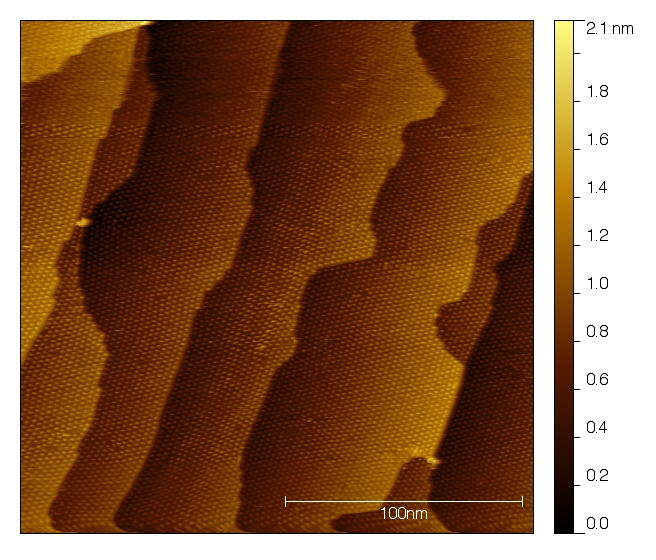
\includegraphics[scale=0.7]{./figs/graphene-ruthenium-stm.png}
  \caption{
  STM image displaying characteristic moire pattern formed by graphene grown atop Ru(0001). The graphene sheet grows in a uniform manner across the monatomic steps in the ruthenium surface.
  }
  \label{fig:ru-graphene-long}
\end{figure}

The graphene/ruthenium system is ideal for the study of graphene on metals as a result of the ease of growth for the carbon adsorbate layers on the ruthenium surface. The moire reconstruction of graphene on ruthenium is easily reproducible with the same periodicity and generally independent of the common growth methods. Graphene on ruthenium grown by CVD, PVD, or graphitization will nearly always adopt the same structure with minimal rotational disorder. Furthermore, this system exhibits a high degree of long range ordering with the graphene sheets growing in a uniform manner across the stepped ruthenium surface for multiple microns up to millimeter scale graphene \cite{ mm-graphene}. Figure \ref{fig:ru-graphene-long} shows a typical STM image of the graphene ruthenium surface with long range order and the characteristic moire structure easily visible as the series of bright and dark spots.

\begin{figure}
  \centering
  \includegraphics[scale=0.7]{./figs/atomic-graphene.png}
  \caption{
  Atomically resolved image of the graphene/Ru(0001) system. The moire unit cell is denoted by the black lines in the figure. The bright spots represent the high points of the corrugated structure.
  }
  \label{fig:atomic-graphene}
\end{figure}


The graphene ruthenium moire pattern appears in STM images as a rippled hexagonal superstructure. The peak-to-peak distance, the moire period, can be measured using line profile analysis and is generally consistent with the reported value of 2.98 nm \cite{march}. The moire structure, as imaged by STM, is a physically corrugated system, that is to say the corrugation is not purely an electronic effect such as fluctuation in charge density. The rippled structure can be considered to be made up of areas of varying carbon-ruthenium interaction strength. The peaks in the STM represent area where the carbon atoms are more weakly bound to the ruthenium surface and thus sit higher from the surface. The low points in the structure represent areas with stronger overlap between the graphene $\pi$ orbitals and the ruthenium $4d$ orbitals. As a result, it has been reported that close up STM images of these two regions appear different. In the peaks of the structure, where the carbon atoms are less strongly bound, atomically resolved STM should image all atoms within the graphene rings. In the low regions, where carbon atoms are strongly bound to the surface, the STM images only every other atom in the graphene ring \cite{march}. An atomically resolved room temperature STM image of graphene on ruthenium is shown in Figure \ref{fig:atomic-graphene} with the unit cell of the moire superstructure also denoted. In this image there is not sufficient detail to resolve differences between the imaged atoms in the high sites compared to the low sites of the moire unit cell. Imaging a smaller area and/or imaging at low temperature may resolve this discrepancy.

Graphene grows epitaxially atop the ruthenium surface with relative ease and forms highly ordered uniform sheets with the characteristic rippled structure. The resulting moire structure is independent of the method of growth, CVD, PVD, or graphitization all result in the same structure. However, if graphene is to be utilized as a scaffold for the growth of other materials, then control over the surface structure may be desired. Also its worth nothing that since the moire structure is closely linked to the bonding between the carbon layer and the ruthenium surface, its possible that modulations of the surface structure may induce unique changes in the electronic structure of the graphene-ruthenium system, however, those changes are beyond the scope of the present research. By altering the graphene growth process we have shown that it is possible to form many different moire structures simultaneously and the resultant material is hereby denoted as polymorphic graphene.

Multiple polymorphic graphene samples have been prepared in our combined UHV growth and analysis chamber; the growth of polymorphic graphene results in distinct signatures visible by LEED and STM indicating differences from the standard model of graphene on ruthenium. The primary difference between standard growth of graphene on ruthenium and the growth of polymorphic graphene is the presence of an atmosphere of atomic hydrogen near the sample surface during the carbon deposition.

\subsection{Growth of Polymorphic Graphene}

Physical vapor deposition growth of polymorphic graphene samples begins with preparation and analysis of the underlying Ru(0001) substrate. The ruthenium crystal is depleted of contaminants by repeated cycles of annealing at 1200 K in a moderate atmosphere of molecular oxygen followed by rapid heating to temperatures above 1800 K to remove residual surface oxygen. This process is repeated until the Auger spectrum indicates a crystal free of sulfur, oxygen, and a sufficiently low carbon concentration. At this point the LEED pattern should have only a sharp Ru p(1x1) pattern. If a p(2x2) pattern is visible then likely the surface is still partially oxidized and heating to 1800 K or higher for 20 seconds should desorb all remaining oxygen. The carbon source for PVD is prepared by outgassing overnight before a beginning the growth procedure. The source will remain clean once outgassed until the next time the system has been vented.


\begin{figure}
  \centering
  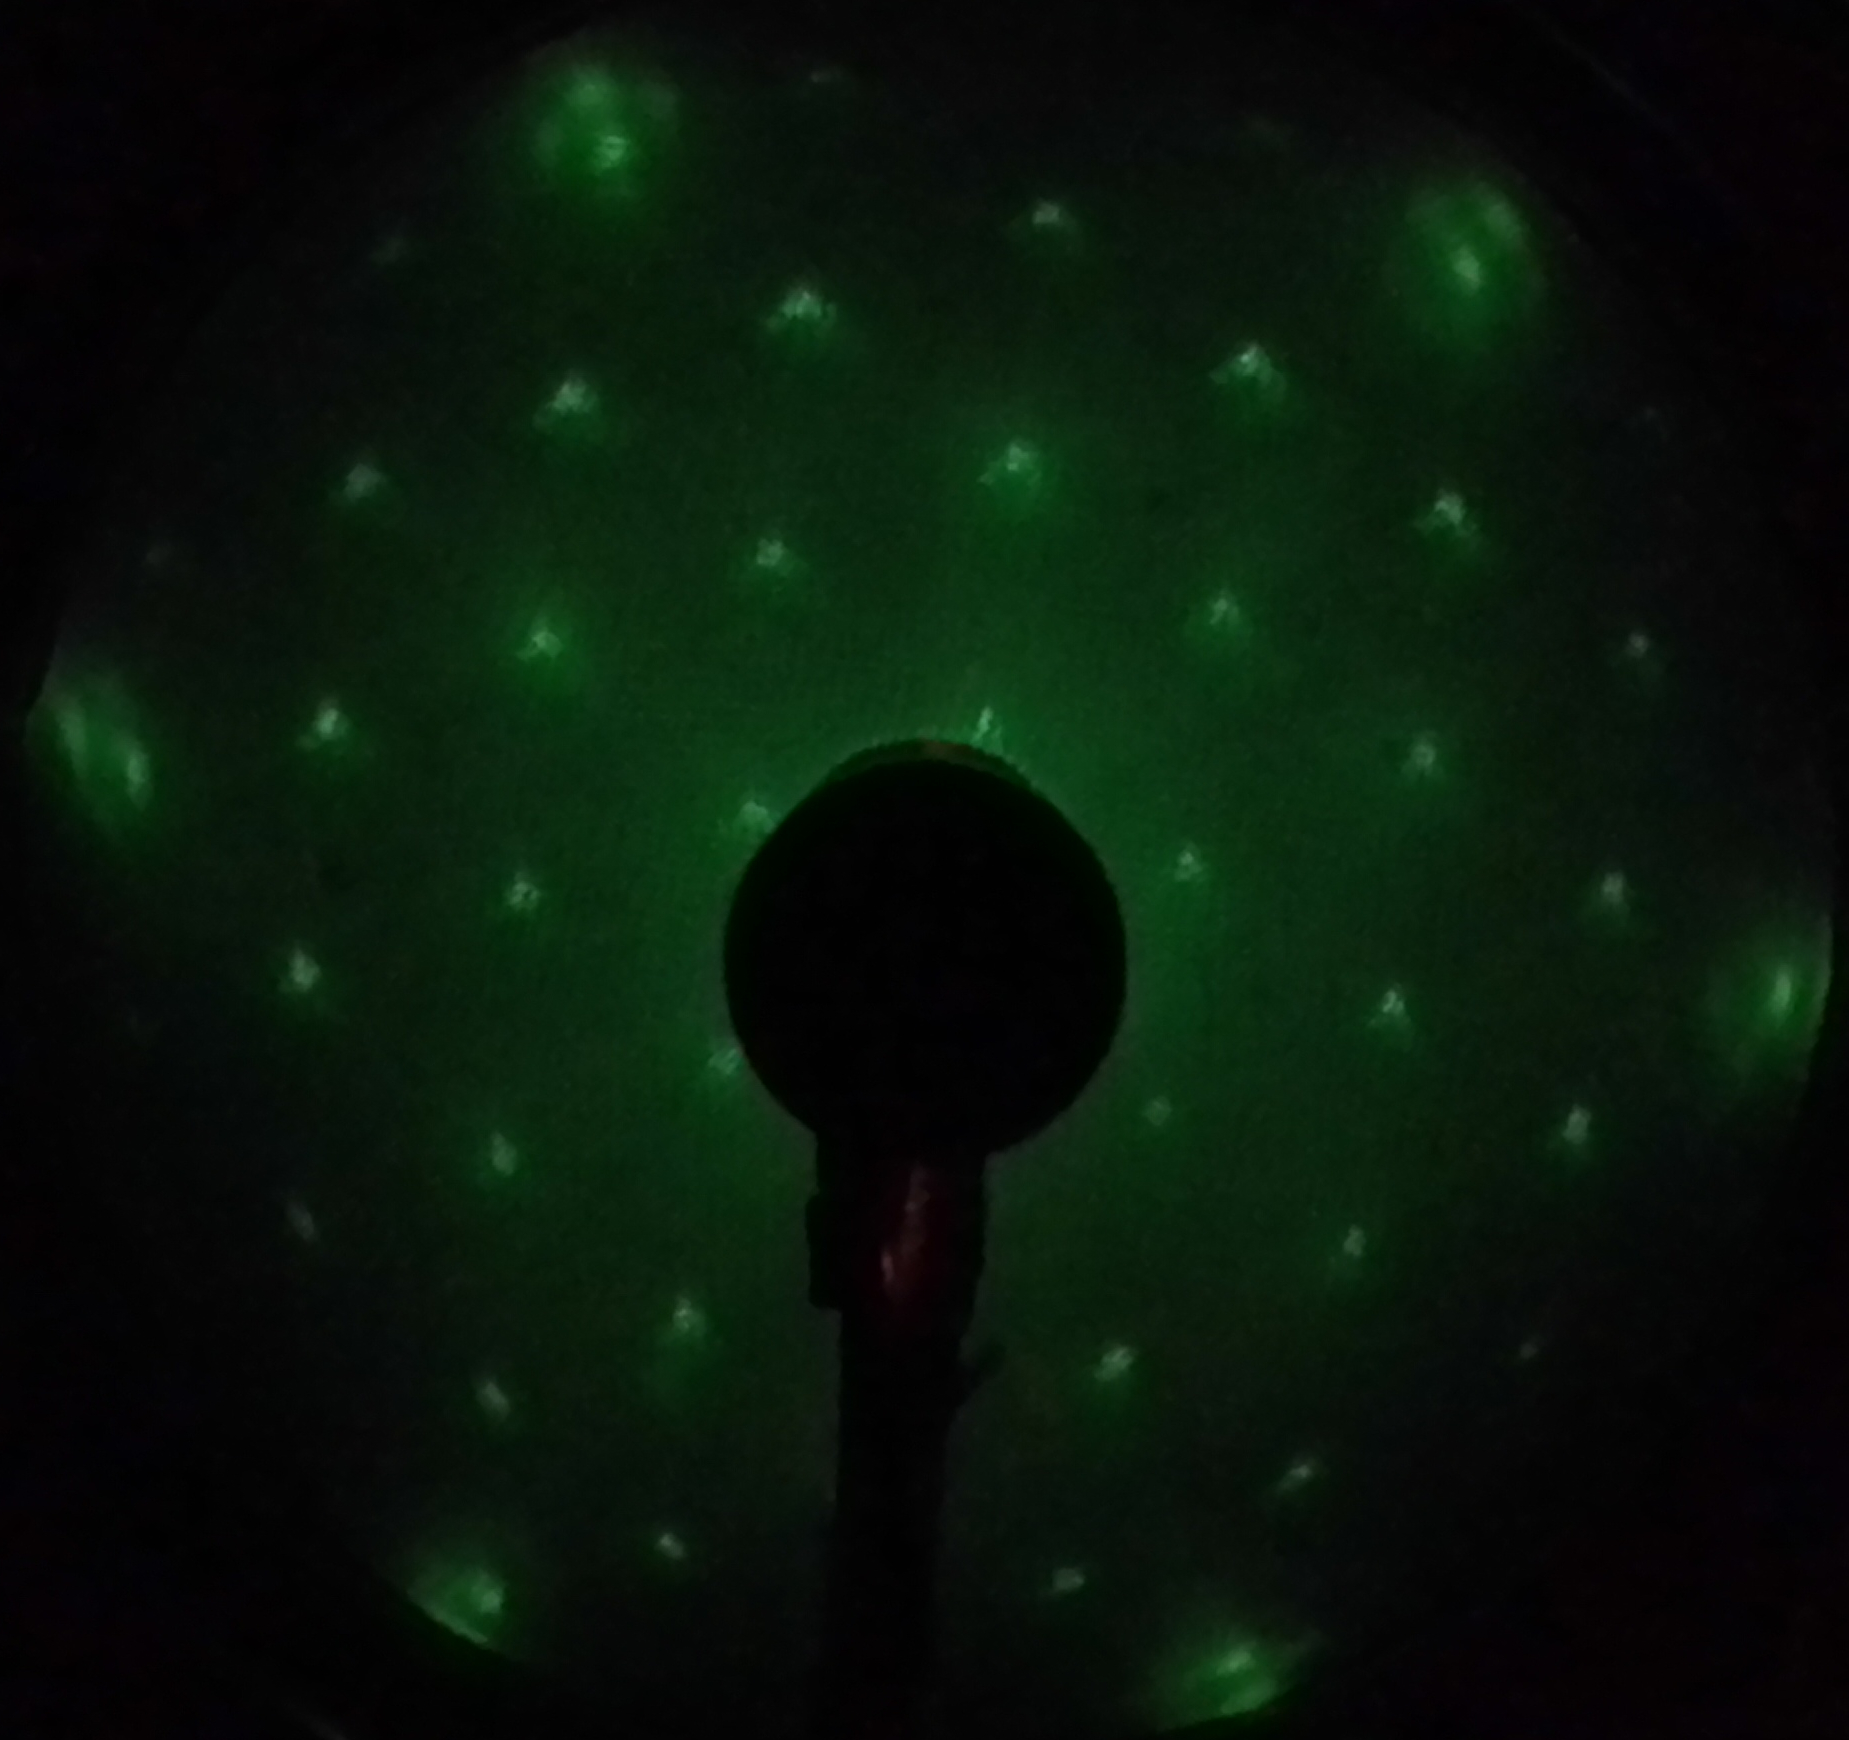
\includegraphics[scale=0.2]{./figs/graphene-hydro-leed.png}
  \caption{
  LEED pattern obtained after a growth of polymorphic graphene on a ruthenium (0001) substrate. Compared with Figure \ref{fig:graphene-leed}, there are many extra diffraction peaks. These peaks form a $(2\sqrt{3}$ x $2\sqrt{3})$R$30^\circ$ pattern relative to the primary Ru (1x1) pattern.
  }
  \label{fig:graphene-hydro}
\end{figure}

The temperature of the crystal and the carbon source are both crucial parameters for the growth process. The carbon source must be hot enough to sublimate carbon atoms to the ruthenium crystal surface as well as hot enough to fracture a hydrogen gas molecule. The temperature of the carbon source can be monitored with an optical pyrometer, whereas the temperature of the ruthenium crystal is monitored both by an optical pyrometer and a C-type thermocouple spot welded to the side of the crystal. The sample crystal should be brought as close to the carbon source as possible; direct line of sight between the carbon source and the sample presents a flux of carbon atoms to the ruthenium surface. A smaller distance between the sample and the source also serves to maximize the local atmosphere of atomic hydrogen gas.

With the sample positioned close to the carbon source, the temperature of the crystal is raised to near 800K by heating with a tungsten filament mounted behind the crystal. After a slight period of preheating the sample, the carbon source is brought up to temperatures above 1800K. At this point the UHV chamber is backfilled with ultra high purity molecular hydrogen to a pressure between $3$x$10^{-7}$ and $1$x$10^{-6}$ torr. The hot carbon source acts as a fracturing element for the atmosphere of molecular hydrogen gas thus creating a local atmosphere of atomic hydrogen in close proximity to the sample surface. This results in an incident flux of carbon atoms and atomic hydrogen onto the ruthenium surface.

The co-deposition process can be carried out for anywhere between 30 to 90 minutes. After halting the deposition, the LEED pattern can be assessed, however, generally an annealing cycle must follow the deposition to generate a clear LEED pattern. After the deposition, the sample is annealed at 1200-1225 K until a clear LEED pattern is obtained. This entire process may need to be repeated several times to achieve the desired sample quality. 

\begin{figure}
  \centering
  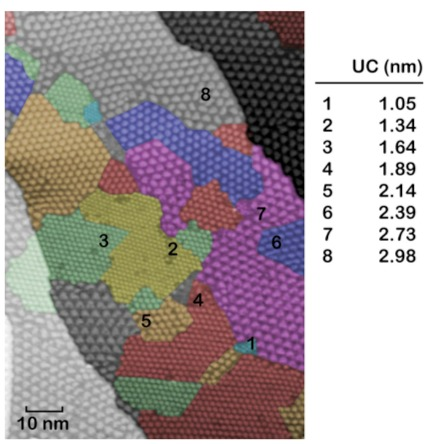
\includegraphics[scale=0.8]{./figs/moires.jpg}
  \caption{STM image displaying multiple domains of graphene with differing periodicity. Eight separate domains, each with a different moire period, are false colored for clarity.}
  \label{fig:polygraphene}
\end{figure}

\section{Polymorphic Graphene: A modulated graphene structure}

The signature of polymorphic graphene can be seen in multiple ways after the deposition. The first indication that the sample is distinct from the standard graphene ruthenium system comes from analysis of the LEED pattern. After co-depostion of atomic hydrogen and carbon, additional LEED spots forming a $(2\sqrt{3}$x$2\sqrt{3})$R$30^\circ$ pattern relative to the Ru p$(1$x$1)$ pattern are visible but often very faint in intensity. The relatively low intensity of the additional LEED spots may indicate that the sample quality is low or that the area exhibiting polymorphism is small. Figure \ref{fig:graphene-hydro} shows the LEED pattern exhibiting extra diffraction peaks alongside the primary ruthenium and moire peaks. Auger spectroscopy confirms that there are no additional contaminants in the sample surface region, thus it can be concluded that the presence of additional LEED peaks stems from the addition of hydrogen to the growth process. Given that conventional LEED displays the reciprocal space LEED pattern averaged over a large sample area, it can not be directly concluded what $(2\sqrt{3}$x$2\sqrt{3})$R$30^\circ$ pattern represents with respect to the physical structure of the system. Thus further analysis of the system is required.

\begin{figure}
  \centering
  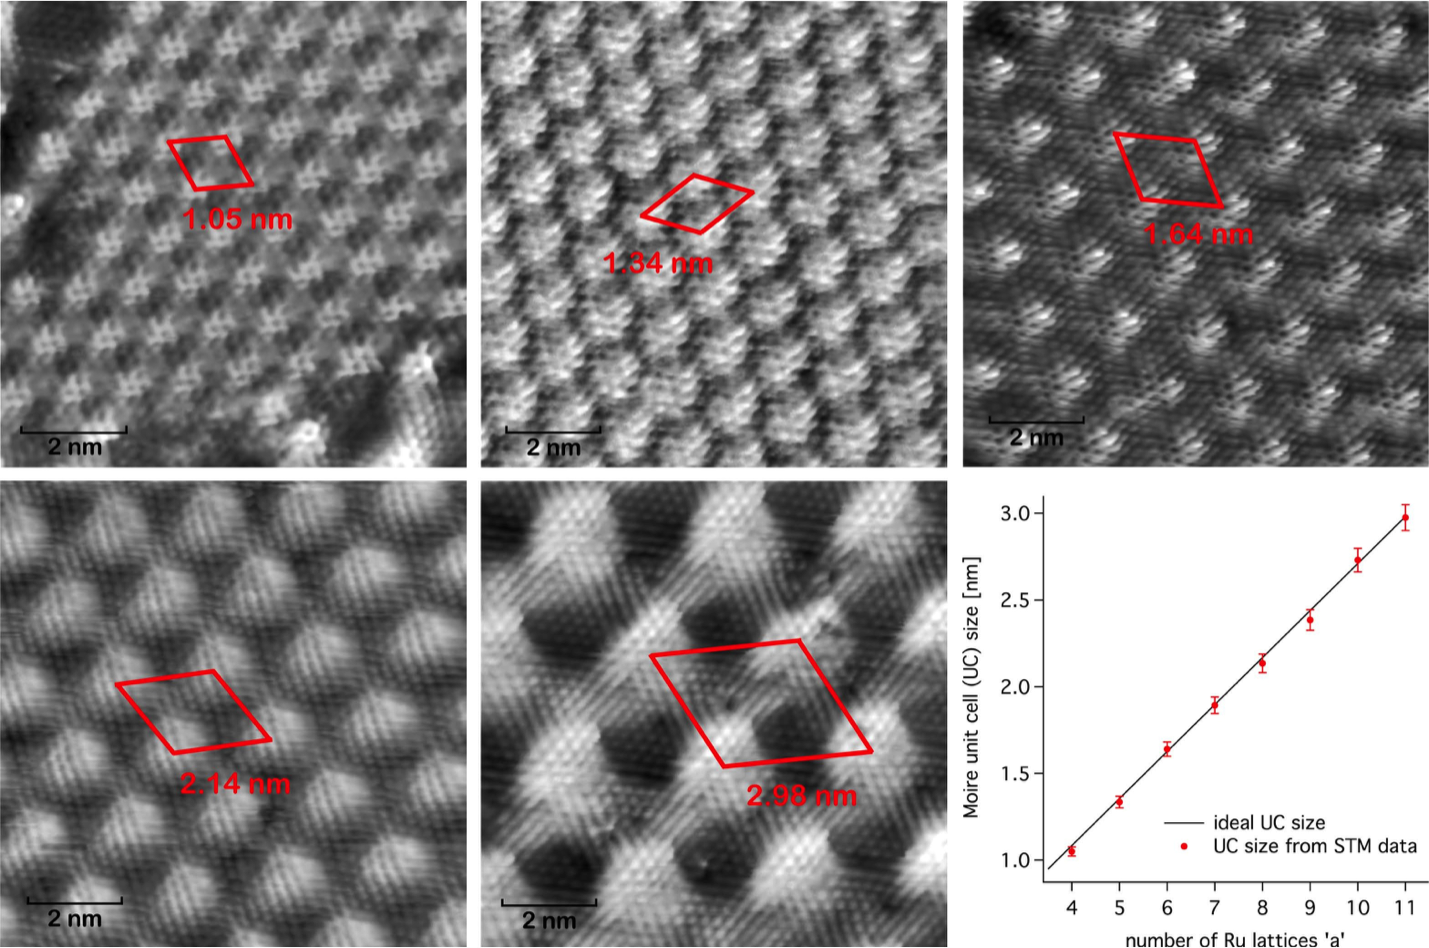
\includegraphics[scale=0.68]{./figs/unit-cell-plot.png}
  \caption{
  Atomically resolved STM images of polymorphic graphene. Domains with different unit cell sizes are shown with a unit cell overlay. Bottom Right: Plotting Moire unit cell size against the number of ruthenium lattices which fit in each unit cell length displays a linear relationship. 
  }
  \label{fig:unit-cell-plot}
\end{figure}

The second indication of structural deviation from the standard graphene/ruthenium system comes from analyzing STM images from the sample surface. STM analysis reveals numerous distinct domains in the graphene surface with a wide range of moire periods. Previously, only moire domains of 2.98 nm and 2.4 nm have been reported from STM investigation of graphene on ruthenium \cite{march, vazquez}. STM images of polymorphic graphene grown using the aforementioned procedure display morie unit cell sizes ranging from 1 nm to the standard value of 2.98 nm covering many values in between but never larger than 2.98 nm. An analysis of moire unit cell sizes observed compared with the number of ruthenium unit cells which fit in a given moire unit cell shows a linear relation between moire unit cell size and number of ruthenium unit cells. This implies that each consecutive moire superstructure corresponds to an increase of superstructure size by one single ruthenium unit cell. Using the previously defined nomenclature for describing the graphene/ruthenium superstructure, this relationship is quantified as follows: for a given moire structure with unit cell size, $a_n$, corresponding to a superstructure consisting of n+1 graphene unit cells atop n ruthenium unit cells, the next largest moire structure will have a moire period of $a_{n+1}$ and a superstructure denoted by n+2 x n+1.

There is some discrepancy as to the exact size of the moire superstructure in the graphene ruthenium system. DFT studies suggest there is little difference energetically when modeling the system as 12x11, 11x10, or other similarly sized superstructures \cite{graphene-metals}. Measurements from conventional LEED generally cannot distinguish between the difference in a 12x11 structure or an 11x10 structure. Taking the ratios between the two observed reciprocal lattice vectors will lead to a value somewhere in between 11 and 12 \cite{graphene-metals}. However, a surface x-ray diffraction, SXRD, experiment remedies the discrepancy with convincing evidence that the true periodic structure in the graphene/ruthenium system is larger by a factor of two \cite{sxrd}. The suggested model for the superstructure is split into four moire sublattices with a total size of 25 graphene unit cells atop 23 ruthenium unit cells. This model can then be envisioned as made up of four of the previously mentioned superstructures if they are accepted to have a superstructure size of 12.5 x 11.5. Using this model, the graphene superstructure is described by n+2 graphene unit cells atop n ruthenium unit cells, (n+2 x n).

\begin{figure}
  \centering
  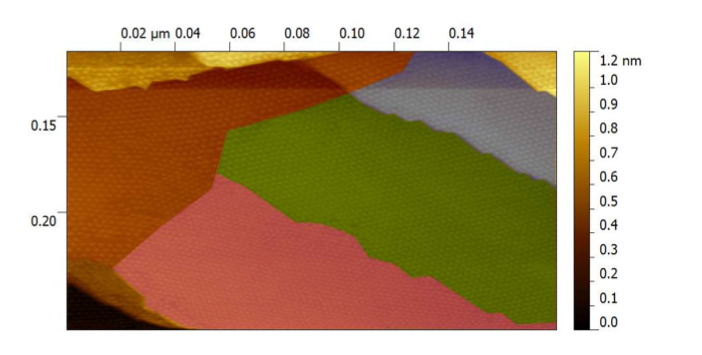
\includegraphics[scale=0.72]{./figs/half-integer-structures.png}
  \caption{
  STM images false-colored to show domains with differing moire periodicities. The green domain has a moire period of 2.56 nm, which corresponding to a (22 x 20) total superstructure consisting of four inequivalent subcells with periods of 2.56 nm. 
  }
  \label{fig:moire25}
\end{figure} 

During STM investigation of a polymorphic graphene sample, additional domains were discovered, which did not fit correctly in the old model for the superstructure size. Figure \ref{fig:moire25} displays a polymorphic graphene domain with a moire period of 2.56 nm. Comparing this value to the plot of unit cell size against number of ruthenium lattices shown in Figure \ref{fig:unit-cell-plot}, its clear that a unit cell size of 2.56nm would have corresponded to fractional values of the total number of ruthenium unit cells contained in the superstructure. A moire period of 2.56 nm would correspond, using the old model, to a (10.5 x 9.5) superstructure. Using this larger scale model suggested by SXRD for the total moire structure, we can fit STM observations of additional moire sizes, which were incompatible with the previous model. If instead the (n+2 x n) model is used, which generates a superstructure size of (25 x 23) for the standard graphene/ruthenium system, then the 2.56 nm moire structure fits a (22 x 20) superstructure that consists of four inequivalent cells with unit cell size of 2.56 nm.

\section{Limitations in analysis of polymorphic graphene}

A number of open questions remain concerning the growth and properties of polymorphic graphene, some of which are beyond the scope of this thesis work, however others will be explored in further chapters. Chief among the list of questions is addressing the role of hydrogen in the polymorphic graphene system. The STM images of the polymorphic graphene surface demonstrate the prospect of modulating the surface structure of the graphene/ruthenium system at the atomic level. The growth process for polymorphic graphene allows many moire domains to nucleate which would be otherwise energetically disfavored. Analysis of the surface of polymorphic graphene with atomic resolution shows little difference from the standard graphene/ruthenium system aside from the change in moire period. From the STM images the possibility that the surface of the graphene system contains hydrogen can be ruled out. In other words, the growth process is not forming graphane, the hydrogenated form of graphene, at least when viewed from the top down. 

One of the limitations of STM characterization is that the imaging technique is only sensitive to the topmost surface layer. Thus while the polymorphic graphene system can be imaged with atomic precision, there is a lack of understanding of the structure of the system below the carbon surface. Comparison of LEED patterns and STM images of standard graphene/ruthenium systems to the polymorphic graphene/ruthenium system show staunch differences, thus the hydrogen modulation of the growth process must play an important role. However, with STM and conventional LEED alone, no data can be obtained as to the role the hydrogen plays in the nucleation of different graphene domains.

Furthermore, STM investigation of the system does not easily provide information concerning the thickness of the carbon layer or layers at the surface. Thus it is not known whether single layer, bilayer, or many layers of graphene are grown atop the ruthenium surface. As mentioned in Chapter 3, low energy electron microscopy, LEEM, allows the surface of a crystal to be imaged simultaneously with an epitaxial growth process. It has been shown that LEEM provides a unique way to observe the nucleation of graphene islands and further growth into large scale graphene sheets atop the ruthenium surface \cite{mccarty-carbon, c-clusters}. Using this method, determination of the layer thickness is relatively straightforward given that the nucleation of each subsequent layer can be observed in real time. There is, however, one major limiting factor that makes using this technique to characterize polymorphic graphene growth more difficult. Currently polymorphic graphene growth happens at mid to high vacuum levels with relatively high pressures of hydrogen gas used relative to the base pressure of a LEEM system. Furthermore, currently polymorphic graphene growth has only been tested using a PVD growth process using a solid carbon source. These two properties of the growth process make integration with a LEEM system difficult, however it may be possible to adapt the growth of polymorphic graphene to a CVD, MBE, or segregation growth process more suitable to integration with LEEM. Chapter 5 will explore an alternative method for addressing the question of carbon layer thickness in the polymorphic graphene samples.

As mentioned before, STM can provide atomic scale images of only the upper most surface layer in the system. No other information concerning atomic positions subsurface is available. It may be of interest to have a better understanding of the precise atomic reconstructions present in polymorphic graphene as applied to the entire superstructure as a whole. To do so, information is needed about the positions of the ruthenium atoms within the supercell as well as the hydrogen. There are a limited number of surface science techniques available that can provide atomic scale information regarding the three dimensional position of atoms in the system with resolution small enough to probe individual domains in the polymorphic graphene system. Chapter 3 discussed LEED-I(V) as one potential tool for mapping atomic positions in a crystalline solid. Specifically LEED-I(V) carried out in a LEEM system has the possibility to restrict the electron beam sample area to sub-micron levels. Thus $\mu$-LEED-I(V) is an ideal candidate for further study of the polymorphic graphene system.

Finally, there are a number of open questions about the properties of polymorphic graphene, which are beyond the scope of this work but may warrant future studies. Specifically this work has focused on the structural characteristics of the polymorphic graphene system and their differences when compared to the standard graphene/ruthenium system. Given that the electronic properties of a material can be inherently linked to the structure of the material, it is quite possible that polymorphic graphene exhibits distinct electronic properties compared to the standard graphene/ruthenium system.

Pristine freestanding graphene is known to be a zero-gap semiconductor with extraordinarily high conductance. However, single layer graphene on ruthenium should depart from freestanding graphene significantly due to the strong overlap in the moire low regions between the graphene $\pi$ orbital and the ruthenium $4d$ orbital. This strong binding should disrupt the structure of graphene $\pi$ bands. Polymorphic graphene, however, may exhibit properties closer to pristine graphene as a result of the hydrogen in the system due to similarities with other graphene systems involving hydrogen. 

Silicon carbide is one of the most commonly used substrates for the study of graphene due to ease of growth. One common technique to prepare large-scale high quality graphene sheets involves the graphitization of 6H-SiC (0001). When a single carbon layer is grown in this manner, it remains strongly bound to the SiC surface, and as such is commonly referred to as a buffer layer, since it will not exhibit graphene like properties. However, it has been shown that when this system is exposed to a flux of atomic hydrogen, the hydrogen atoms penetrate the carbon surface layer and bind strongly at the SiC interface \cite{ SiC-passivation}. This is a result of the numerous dangling bonds present at the SiC interface. The hydrogen atoms passivate the SiC surface, which has a number of results. First it drastically reduces the total surface energy at the interface between SiC and the carbon buffer layer. Finally, the carbon buffer layer is lifted up higher from the SiC surface and becomes very weakly bound to the surface. Thus this process of hydrogen passivation transforms the strongly bound carbon layer into what is now called quasi-freestanding epitaxial graphene.

The graphene/ruthenium system may have a similar reaction to hydrogen intercalation. Initially there is strong bonding between carbon and ruthenium in the low points of the moire superstructure. The corrugated moire superstructure also presents many ruthenium dangling bonds at the interface between the ruthenium surface and the carbon layer. When atomic hydrogen is introduced into the system its possible that the hydrogen penetrates the carbon surface and remains bound at the interface between ruthenium and graphene. It has been previously mentioned that there is no indication found of hydrogen atop the carbon surface layer. Thus if hydrogen remains present in the system after the growth process, it must be at least subsurface relative to the uppermost carbon layer. If the atomic hydrogen manifests at the carbon-ruthenium interface, then it should be expected that the carbon surface layer is lifted higher from the ruthenium surface in a similar manner to the silicon carbide system. If this is the case then it can be expected that the electronic properties of this system will be different from those of the standard graphene/ruthenium system as a result of weaker overlap between the passivated ruthenium and carbon. These properties could be explored in the future using a combination of scanning tunneling spectroscopy, STS, and micro spot sized angle resolved photoemission spectroscopy, $\mu$-ARPES, to better understand the density of states and band structure of the system. ARPES measurements have been carried out for the graphene/ruthenium system before and after intercalation of atomic oxygen and the results are similar to those of the graphene/SiC system when exposed to atomic hydrogen \cite{o2-intercalation}. 




